\documentclass[a1paper,landscape,american,11pt]{baposter}

\usepackage{lipsum}
\usepackage{tikz}
\usetikzlibrary{
    arrows,
    arrows.meta,
    backgrounds,
    calc,
    chains,
    decorations,
    decorations.pathreplacing,
    matrix,
    positioning,
    scopes,
    shadows,
    shapes,
    shapes.multipart,
}

\definecolor{MyColorOne}{HTML}{637462}
\definecolor{MyColorTwo}{HTML}{b7af8a}
\definecolor{MyColorThree}{HTML}{ccb15a}

\tikzstyle{rect}=[draw,rectangle,thick,on chain,font=\tiny,inner sep=1mm,minimum height=1.25em]

\begin{document}
\begin{poster}{
        % Poster Settings
        background=none,
        % Box Settings
        boxColorOne=white!96!black,
        %boxColorOne=MyColorTwo!30!white,
        %boxColorTwo=MyColorThree!30!white,
        %boxshade=shadeTB,
        boxshade=plain,
        headershade=shadeLR,
        headerColorOne=MyColorOne,
        headerColorTwo=MyColorTwo,
        textborder=none,
        headerborder=none,
        headershape=roundedright,
        headerfont=\large\bfseries,
        headerFontColor=white!90!MyColorTwo,
        linewidth=0pt,
    }
    {}
    {
        ACM~SIGMOD'19~Programming~Contest
    }
    {
        \vspace*{.5em}
        \bfseries
        \emph{teamsic:}~Immanuel~L.~Haffner
    }
    {
    }

    \headerbox{Task Description}{name=task,column=0,span=2}{
        \includegraphics[scale=.25]{fig/task_overview.jpg}

        \begin{center}
            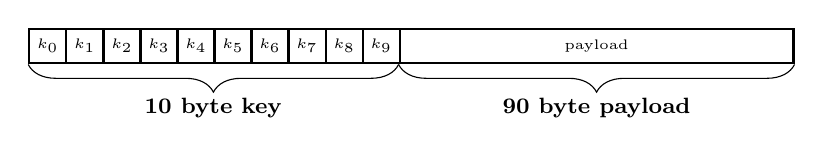
\begin{tikzpicture}
                \begin{scope}[start chain=going right,node distance=-\pgflinewidth]
                    \node[rect] (k0) {$k_0$};
                    \node[rect] {$k_1$};
                    \node[rect] {$k_2$};
                    \node[rect] {$k_3$};
                    \node[rect] {$k_4$};
                    \node[rect] {$k_5$};
                    \node[rect] {$k_6$};
                    \node[rect] {$k_7$};
                    \node[rect] {$k_8$};
                    \node[rect] {$k_9$};
                    \node[rect,minimum width=50mm] (payload) {payload};
                    \draw[decorate,decoration={brace,mirror,amplitude=10pt}]
                    (k0.south west) -- node[below=3mm] {\footnotesize\textbf{10 byte key}} (payload.south west);
                    \draw[decorate,decoration={brace,mirror,amplitude=10pt}]
                    (payload.south west) -- node[below=3mm] {\footnotesize\textbf{90 byte payload}} (payload.south east);
                \end{scope}
            \end{tikzpicture}
        \end{center}

        \begin{itemize}
            \item 2x Intel Xeon E5-2640v4 @2.4GHz (10 cores, 20 hypterthreads, 25\,MiB cache, AVX-2)
            \item 30\,GiB RAM
            \item Ubuntu 17.10 with Linux 4.13
            \item 2 1.6\,TB SATA-6GBPS SSD (500\,MB/s read, 475\,MB/s write)
        \end{itemize}
    }

    \headerbox{Sorting Algorithm}{name=algo,column=2,span=2}{
        \lipsum[2]
    }

    \headerbox{In-Memory Sorting}{name=inmemory,column=0,span=2,below=task}{
        \lipsum[3]
    }

    \headerbox{External Memory Sorting}{name=external,column=2,span=2,below=algo}{
        \includegraphics[scale=.20]{fig/timeline.png}
    }
\end{poster}
\end{document}
